\documentclass[11pt,a4paper]{article}
\usepackage{polski}
\usepackage[utf8]{inputenc}
\usepackage{geometry}
\usepackage{graphicx}
\usepackage[dvipsnames]{xcolor}

\newgeometry{tmargin=3cm, bmargin=3cm, lmargin=1cm, rmargin=1cm}

\title{Testy aplikacji}
\author{Damian Rakowski 209300}
\date{12 czerwiec 2019}
\newcommand{\testA}{\textcolor{blue}{\textbf{Spodziewany rezultat:\quad}}}
\newcommand{\testB}{\textcolor{blue}{\textbf{Rzeczywiste działanie:\quad}}}
\newcommand{\testT}{\textcolor{green}{\large{\textbf{TEST ZALICZONY}}}}
\newcommand{\testN}{\textcolor{red}{\large{\textbf{TEST NIEZALICZONY}}}}
\newcommand{\testM}{\textcolor{purple}{\large{\textbf{TEST NIEJEDNOZNACZNY}}}}

\begin{document}
\maketitle
\section{Wygląd aplikacji}
\begin{figure}[h]
\centering
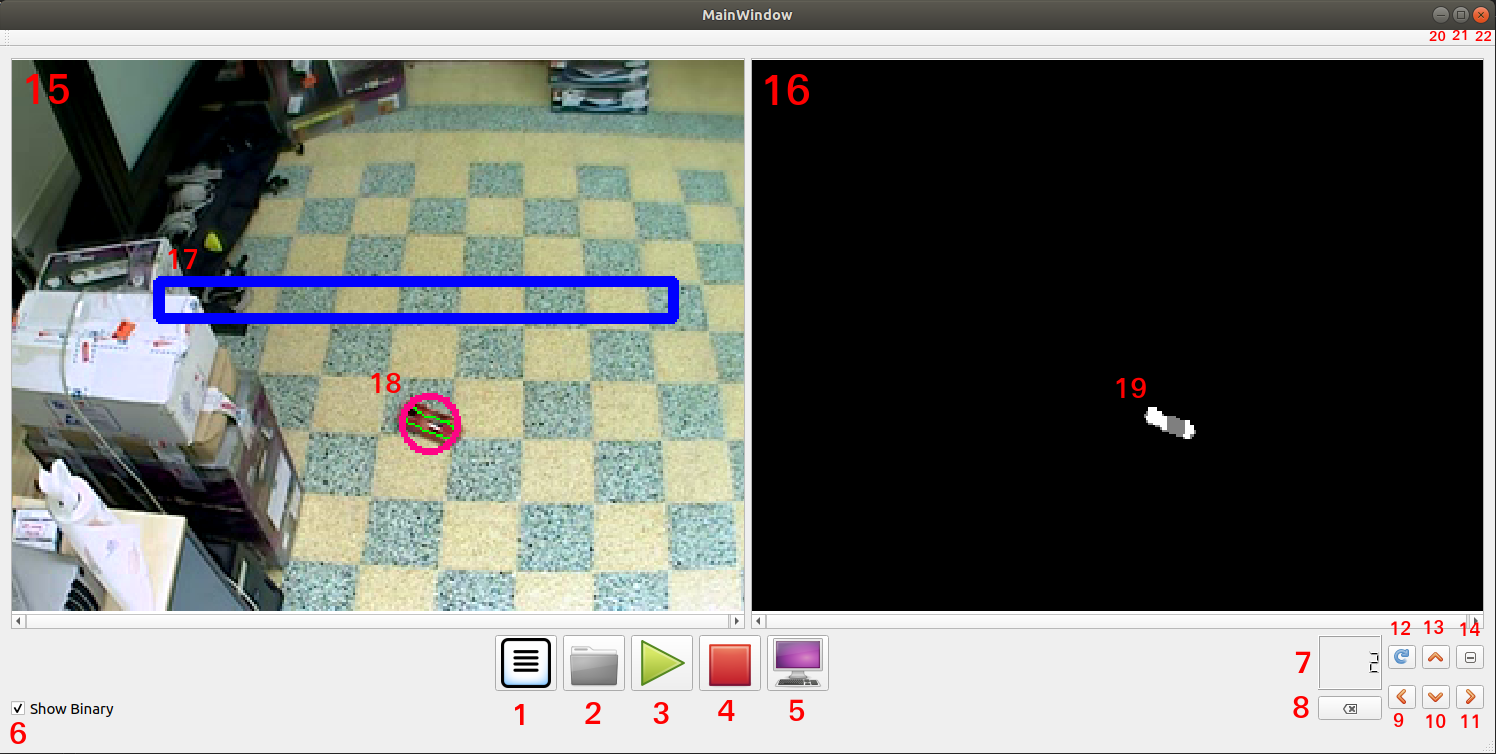
\includegraphics[width=\textwidth]{aplikacja.png}
\caption{Aplkiacja główna}
\vspace{1.5cm}
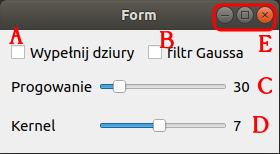
\includegraphics[scale=1]{opcje.png}
\caption{okienko z opcjami algorytmu}
\end{figure}

\section{Funkcjonalności do przetestowania manualnego}
\begin{enumerate}
\item[1] aplikacja wczytuje i odtwarza pliki avi,mp4,webm na ekranie (15). 
\item[2] wstrzymywanie/ponowne uruchamianie/zamykanie pliku wideo (3,4)
\item[3] wykryty  obiekt na obrazie jest opisany na  różowym kręgu oraz wyświetlane są jego krawędzie w kolorze zielonym (15,16)
\item[4] otwieranie/zamykanie obrazu binarnego (16)
\item[5] przetwarzanie pliku z kamery internetowej (5)
\item[6] otwieranie/zamykanie widżetu z parametrami algorytmu (1)
\item[7] zmiana położenia/rotacji/długości bramki wirtualnej przyciskami (12,13,14,9,10,11,17)
\item[8] zmiana położenia/rotacji/długości bramki wirtualnej klawiszami A/W/S/D/R/T
\item[9] bramka zlicza ruchomy obiekt, który przejechał przez bramkę i wyświetla wynik w 7.
\item[10] bramka zmienia kolor w zależności od wykrytego obiektu w środku
\item[11] Aplikacja nie pozwoli wczytać pliku innego niż video i wyświetli ostrzeżenie
\end{enumerate}

\section{Funkcjonalności do przetestowania automatycznego}
\begin{itemize}
\item ustawianie parametrów aplikacji w dodatkowym widżecie
\end{itemize}

\section{Testy manualne}
\begin{enumerate}
\item[1] Wcisnąłem przycisk (2),wczytałem plik .avi i wcisnąłem przycisk (3)\\
\testA aplikacja wczyta plik avi i uruchomi go na ekranie\\
\testB aplikacja wczytała plik avi i uruchmiła go na ekranie

Wcisnąłem przycisk (2), wczytałem plik .mp4 i wcisnąłem przycisk (3)\\
\testA aplikacja wczyta plik mp4 i uruchomi go na ekranie\\
\testB aplikacja wczytała plik mp4 i uruchmiła go na ekranie

Wcisnąłem przycisk (2), wczytałem plik .webm i wcisnąłem przycisk (3)\\
\testA aplikacja wczyta plik webm i uruchomi go na ekranie\\
\testB aplikacja wczytała plik webm i uruchmiła go na ekranie

\testT

\item[2] Wczytałem plik .avi, a następnie wciskałem p.(3) trzy razy w odstępie kilku sekund. Na koniec wcisnąłem p.(4)\\
\testA plik video po pierwszym wciśnięciu p.(3) zostanie odtworzony. Po drugim wciśnięciu p.(3) obraz (15) się zatrzyma, a po trzecim wcisnięciu p.(3) plik video zostanie odtworzony w miejscu, w którym został zatrzymany. Wciśnięcie przycisku p.(4) zatrzyma obraz i zablokuje przycisk p.(3).\\
\testB Wciskanie p.(3) zatrzymywało lub wznawiało odtwarzanie pliku na obrazie (15). Wciśnięcie p.(4) spowodowało zatrzymanie odtwarzania, a p.(3) został zablokowany.\\
\testT
\item[3] Otworzyłem i uruchomiłem plik o nazwie test.avi\\
\testA Wykryty ruchomy obiekt zostanie opisany na różnowym okręgu, a jego kontury staną się zielone.\\
\testB Ruchomy samochodzik został opisany na różowym okregu, a jego kontury stały się zielone.

Uruchomiłem plik o nazwie test2.mp4.\\
\testA Wykryty ruchomy obiekt zostanie opisany na różnowym okręgu, a jego kontury staną się zielone.\\
\testB Aplikacja wykrywała smochody, odbicia świateł  oraz cienie.\\ Niektóre samochody były traktowane jako zbiór kilku ruchomych obiektów.

\testM

\item[4] Uruchomiłem plik test.avi, a następnie zaznaczyłem pole (6). Po paru sekundach odznaczyłem pole (6).\\
\testA Zaznaczenie p.(4) spowoduje pojawienie się nowego okna z obrazem binarnym po prawej stronie aplikacji. Odznaczenie p.(6) spowoduje zamkniecie binarnego obrazu po prawej stronie aplikacji\\
\testB Po zaznaczeniu p.(6), pojawił się obraz binarny po prawej stronie aplikacji. Kiedy odznaczyłem p.(6), to obraz binary znikł.\\
\testT
\item[5]  Uruchomiłem aplikację i wcisnąłem p.(5).\\
\testA Na ekranie (15) pojawi się obraz z kamery, który jest przetwarzany w czasie rzeczywistym.\\
\testB Na ekranie (15) pojawił się obraz z kamery, na którym pojawiały się okręgi oraz zielone kontury\\
\testT
\item[6] Po uruchomieniu aplikacji wcisnąłem p.(1). Wyskoczyło okienko, które zamknąłem i ponownie wcisnąłem p.(1)\\
\testA Przyciśniecie p.(1) spowoduje wyświetlenie okienka z parametrami, które monża zamknąć i wyswietlić ponownie za pomocą p.(1)\\
\testB Po przyciśnięciu p.(1) wyświetliło się okienko, które zamknąłem krzyżykiem i wyświetliłem ponownie za pomocą p.(1).\\
\testT
\item[7] Uruchomiłem aplikację oraz odtworzyłem plik test.avi. Nastepnie, wcisnąłem p.(14).\\
\testA Wciśnięcie p.(14) spowoduje pojawienie się wirtualnej bramki w lewym górnym rogu\\
\testB W prawym górnym rogu pojawił się niebieski prostokąt.

Uruchomiłem aplikację oraz odtworzyłem plik test.avi. Nastepnie, wcisnąłem p.(14) i p.(11)\\
\testA Pojawi się wirtualna bramka, która przesunie się w prawo.\\
\testB Niebieska bramka przesunęła się w prawo.

Uruchomiłem aplikację oraz odtworzyłem plik test.avi. Nastepnie, wcisnąłem p.(14) i p.(10)\\
\testA Pojawi się wirtualna bramka, która przesunie się w dół.\\
\testB Niebieska bramka przesunęła się w dół.

Uruchomiłem aplikację oraz odtworzyłem plik test.avi. Nastepnie, wcisnąłem p.(14), p.(11) i p(9)\\
\testA Pojawi się wirtualna bramka, która przesunie się w prawo, a nastepnie wróci do swojeje pozycji.\\
\testB Niebieska bramka przesunęła w prawo, a na następnie w lewo.

Uruchomiłem aplikację oraz odtworzyłem plik test.avi. Nastepnie, wcisnąłem p.(14), p.(10) i p(13)\\
\testA Pojawi się wirtualna bramka, która przesunie się w dół, a nastepnie wróci do swojeje pozycji.\\
\testB Niebieska bramka przesunęła w dół,a  na następnie w górę.

Uruchomiłem aplikację oraz odtworzyłem plik test.avi. Nastepnie, wcisnąłem p.(14) i p.(12)\\
\testA Pojawi się wirtualna bramka, która obróci się o 90 stopni.\\
\testB Niebieska bramka z pozycji horyzontalnej przeszła w pozycję pionową.

\testT


\item[8] Uruchomiłem aplikację oraz odtworzyłem plik test.avi. Nastepnie, wcisnąłem klawisz T.\\
\testA  Pojawi  się wirtualna bramka w lewym górnym rogu\\
\testB W prawym górnym rogu pojawił się niebieski prostokąt.

Uruchomiłem aplikację oraz odtworzyłem plik test.avi. Nastepnie, wcisnąłem kla. T  i kla. D\\
\testA Pojawi się wirtualna bramka, która przesunie się w prawo.\\
\testB Niebieska bramka przesunęła się w prawo.

Uruchomiłem aplikację oraz odtworzyłem plik test.avi. Nastepnie, wcisnąłem kla. T i kla. S\\
\testA Pojawi się wirtualna bramka, która przesunie się w dół.\\
\testB Niebieska bramka przesunęła się w dół.

Uruchomiłem aplikację oraz odtworzyłem plik test.avi. Nastepnie, wcisnąłem kla. T, kla. D i kla. A\\
\testA Pojawi się wirtualna bramka, która przesunie się w prawo, a nastepnie wróci do swojeje pozycji.\\
\testB Niebieska bramka przesunęła w prawo, a na następnie w lewo.

Uruchomiłem aplikację oraz odtworzyłem plik test.avi. Nastepnie, wcisnąłem kla. T, kla. S i kla. W\\
\testA Pojawi się wirtualna bramka, która przesunie się w dół, a nastepnie wróci do swojeje pozycji.\\
\testB Niebieska bramka przesunęła w dół,a  na następnie w górę.

Uruchomiłem aplikację oraz odtworzyłem plik test.avi. Nastepnie, wcisnąłem kla. T i kla. R\\
\testA Pojawi się wirtualna bramka, która obróci się o 90 stopni.\\
\testB Niebieska bramka z pozycji horyzontalnej przeszła w pozycję pionową.

\testT

\item[9] Otworzyłem plik test.avi i ustawiłem wirtualną bramkę na środku obrazu, na całej szerokości.\\
\testA Za każdym razem kiedy samochodzik przejedzie przez bramkę, licznik (7) wzrasta o 1.\\
\testB Kiedy samochodzik przejeżdzał przez bramkę, wartość licznika rosła o 1.\\
\testT

\item[10]  Otworzyłem plik test.avi i ustawiłem wirtualną bramkę na środku obrazu, na całej szerokości.\\
\testA Kiedy samchodzik znajdzie się wewnątrz bramki, to zmieni ona swój kolor na zielony. Jeżeli samochodzik wyjedzie z bramki, to jej kolor stanie się niebieski.\\
\testB Bramka zmieniała swój kolor z niebieskiego na zielony, jeżeli w środku znajdował się samochodzik.
\testT
\item[11]
Wcisnąłem przycisk (1), a nastepnie wybrałem plik tekstowy i wcisnąłem przycisk wczytaj.\\
\testA Aplikacja wyświetli ostrzeżenie o niepoprawnym formacie wczytywanego pliku.\\
\testB Wyświetliło się ostrzeżenie o niewłaściwym typie pliku
\end{enumerate}



\end{document}
